
\documentclass[12pt]{article}
\usepackage[a4paper, margin=.30in]{geometry}
\usepackage{graphicx ,
            wrapfig,
            xcolor, 
            enumerate,
            amsmath,
			fontenc,
			tcolorbox,circuitikz
            }

\newcommand\headerMe[2]{\noindent{}#1\hfill#2}
\renewcommand{\thesection}{\Roman{section}}

\author{Zakaria HAOUZAN}
\date{\today}

\begin{document}
% headers --------------
\headerMe{Matière : Physique-Chimie}{Professeur : Zakaria HAOUZAN}\\
\headerMe{Unité : Electricité }{Établissement : Lycée SKHOR qualifiant}\\
\headerMe{Niveau : 2BAC-SM-PC}{Heure : 6H}\\

% ------Content ________
\begin{center}

    \Large{Leçon $N^{\circ} 7 $: \color{red} Dipôle RL }
\end{center}

%\begin{wrapfigure}[10]{r}{0.5\textwidth}
%    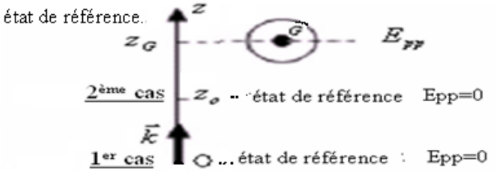
\includegraphics[width=0.5\textwidth]{./img/img00.png}
%\end{wrapfigure}

\section{La Bobine : }
\subsection{Définition : }

 Une bobine est constituée d'un enroulement sur un cylindre dans le même sens d'un fil conducteur recouvert d’un vernis
isolant. , c'est un dipôle inactif (qui joue le rôle d'un récepteur dans un circuit électrique)

\begin{center}
	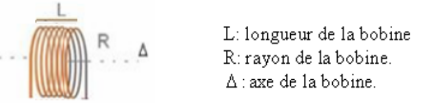
\includegraphics[width=0.5\textwidth]{./img/def_bobine.png}
\end{center}

La bobine est caractérisée par sa résistance interne exprimée en ohm $\Omega$ et par son inductance L exprimée en Henry (H)

\begin{tcolorbox}
	Remarque : 

L'inductance d'une bobine dépend de sa section S ,de sa longueur L et de son nombre N de spires ainsi
que du milieu dans laquelle elle se trouve.

La présence d’un noyau de fer ou d’acier plus ou moins enfoncé dans la bobine permet d’augmenter ou de diminuer
son inductance L : on a ainsi une bobine d’inductance L réglable.
\end{tcolorbox}

\begin{center}
	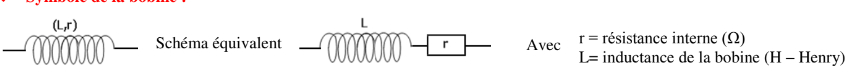
\includegraphics[width=0.8\textwidth]{./img/symboleBobine.png}
\end{center}


En convention récepteur, l'intensité i du courant et la tension uL aux bornes de la bobine sont représentées par
des flèches de sens contraires.

\subsection{Tension aux bornes de la bobine: }
La tension aux bornes d'une bobine d'inductance L et de résistance r parcourue par un courant électrique d'intensité i est donnée par la relation suivante : 
$$u_L = r.i + L.\frac{di}{dt}$$

Si le courant électrique est continue l'intensité du courant est constante donc $\frac{di}{dt} = 0$  alors $u_L =r.I$

\begin{tcolorbox}
La bobine se comporte comme un conducteur ohmique dans le courant continue.
\end{tcolorbox}

\subsection{Détermination expérimentale de l'inductance d'une bobine: }

Expérience: On réalise le montage suivant en utilisant un générateur GBF de signal triangulaire:

avec La sensibilité horizontale utilisée est : $S_H = 0,5ms/ div$ , 

la sensibilité verticale pour Y1 $S_V1 =0,05V / div$ et Y2: $S_V2 = 1.V / div$.
\vspace{1cm}

\textbf{Interprétation:}

A partir du circuit on a $u_1 = u_L = L.\frac{di}{dt}$ car la résistance de la bobine r=0. et $u_2 = -u_R $ donc $i = \frac{-u_2}{R}$

en remplaçant dans u1, elle deviant: $u_1 = -\frac{L}{R}.\frac{du_2}{dt}$

$$L = -\frac{u_1.R}{\frac{du_2}{dt}}$$

\begin{wrapfigure}[1]{r}{0.2\textwidth}
	\vspace{-2cm}
	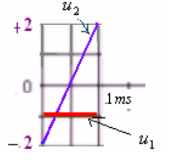
\includegraphics[width=0.2\textwidth]{./img/LBobine.png}
\end{wrapfigure}


Les deux tensions sont périodiques. Il suffit donc de considérer l'intervalle $[0, \frac{T}{2}]$ pour déterminer la valeur de L. On a T = 0,5ms/div*4div = 2ms donc [0,0,1ms]

et dans cet intervalle,  On a $\frac{du_2}{dt} = \frac{u_{2max} - u_{2min}}{\frac{T}{2} - 0} = 4.10^3 V/s$

et $u_1$ = -1div*0,05V/div = -0,05V donc L = 0,25H

\subsection{Influence de la bobine sur le passage du courant dans un circuit:}

\begin{wrapfigure}[6]{r}{0.3\textwidth}
	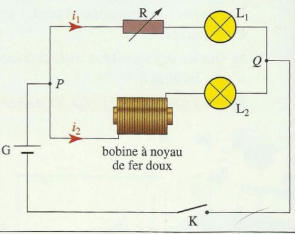
\includegraphics[width=0.3\textwidth]{./img/montage00.png}
\end{wrapfigure}


\textbf{Expérience: }

On réalise le montage expérimental suivant dans lequel les deux lampes sont
identiques et la résistance de la bobine et celle du conducteur ohmique ont la même valeur r=R.


\textbf{Observations: }On constate que 

\begin{itemize}
	\item La lampe L1 brille après la lampe L2 avec un retard de quelques secondes à la fermeture et à l'ouverture de l'interrupteur.

	\item Et en régime permanent les deux lampes brillent de façon identique.

\end{itemize}

\textbf{Interprétations: }On sait que la tension aux bornes de la bobine $u_L = r.i + L.\frac{di}{dt}$

\begin{itemize}
	\item Lorsqu'on ferme l'interrupteur: pendant l'établissement du courant de 0 à I, $L.\frac{di}{dt} > 0$ il retarde l'établissement du courant.

	\item Lorsqu'on ouvre l'interrupteur: pendant l'annulation du courant (de I à 0),$L.\frac{di}{dt} < 0$ il retarde la rupture du courant.

	\item En régime permanent (i = constante), on a alors: $\frac{di}{dt} = 0$ la bobine se comporte comme un conducteur ohmique de résistance r.

\end{itemize}

\begin{tcolorbox}

	Conclusion:

La bobine s'oppose à l'établissement et à l'annulation du courant électrique, cet effet se manifèste lorsque l'intensité
du courant varie (c'est à dire pendant l'ouverture et la fermeture de l'intérrupteur).
\end{tcolorbox}


\section{Réponse d'un dipôle RL à un échelon de tension : }

\subsection{Réponse d'un dipôle RL à un échelon montant de tension:  (Etablissement de courant)}

\begin{wrapfigure}[6]{r}{0.3\textwidth}
	\vspace{-1cm}
	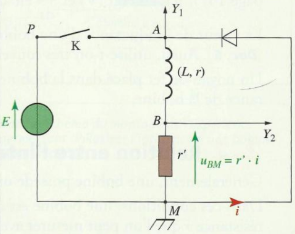
\includegraphics[width=0.3\textwidth]{./img/reponse_RL.png}
\end{wrapfigure}


On monte en série un conducteur ohmique de résistance R et une bobine d'inductance L et de résistance r
auquel on applique un échelon montant de tension à l'aide un générateur de tension en fermant
l'intérrupteur à t=0.

\textbf{Equation différentielle:}

En appliquant la loi d'additivité des tensions on a $u_R + u_L = E$ avec $u_R = R.i$ et $u_L = r.i + L.\frac{di}{dt}$ avec $R_T = R + r$
$$\frac{L}{R_T}.\frac{di}{dt} + i  = \frac{E}{R_T}$$ On pose $\tau = \frac{L}{R_T}$ (constante de temps du dipôle RL).
$$\tau .\frac{di}{dt} + i  = \frac{E}{R_T}$$


\textbf{Solution de l'équation différentielle:}

La Solution de cette équation différentielle est de la forme $i(t) = A.e^{-\alpha.t} + B$ sa derivée $\frac{di}{dt} = -A\alpha.e^{-\alpha.t}$

Les Constantes A,B et $\alpha$ se déterminent en remplaçant et utilisant les conditions initiales.

Donc la solution de l'équation différentielle est : $i(t) = \frac{E}{R_T}(1-e^{-t/\tau})$

\begin{center}


	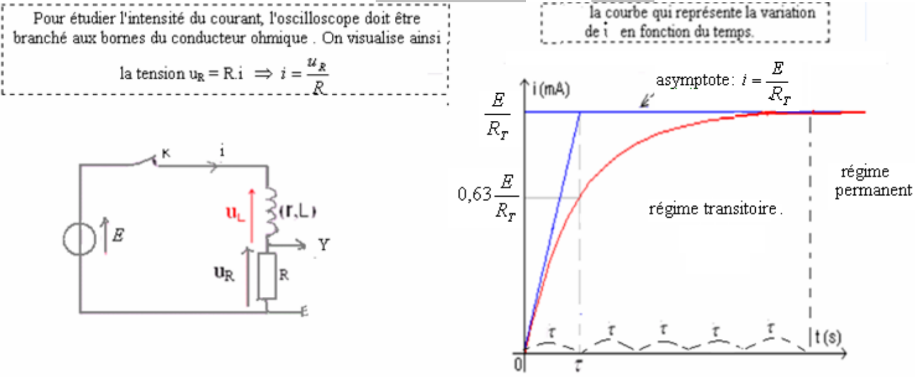
\includegraphics[width=0.9\textwidth]{./img/solution.png}
\end{center}
On constate l'existence de deux régimes:
\begin{itemize}
	\item Un régime transitoire durant lequel l'intensité du courant électrique croit de 0 à I.
	\item Un régime permanent au cours duquel l'intensité du courant électrique devient constante : $i = \frac{E}{R_T}$
	\item Au bout de $5\tau$ le courant électrique s'établit dans la bobine. 
\end{itemize}

\subsection{Unité de la constante de temps: }
On a $\tau = \frac{L}{R_T}$ donc $[\tau] = \frac{L}{R_T}$

avec $u_R = R.i$ et $u_L = L.\frac{di}{dt}$

$$[\tau] = \frac{U.t}{I}.\frac{I}{U} = [t]$$

\subsection{Détermination graphique de la valeur de: $\tau$}


1 ère méthode: En remplaçant dans l'expression de l'intensité $t=\tau$ on obtient $i(t=\tau) = 0,63\frac{E}{R_T}$

Puis par lecture graphique, le temps correspondent à cette valeur est $t = \tau$

2 ème méthode: La tangente à la courbe à t=0 .


\subsection{ Expression de la tension aux bornes de la bobine:}

\begin{center}


	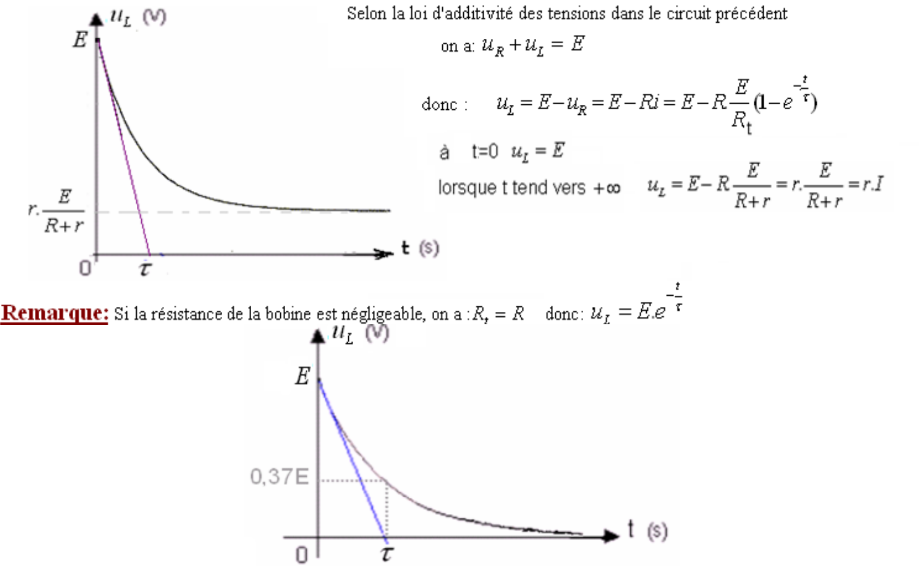
\includegraphics[width=0.9\textwidth]{./img/uLBobine.png}
\end{center}


\subsection{Réponse d'un dipôle RL à un échelon descendant de tension:  (Rupture (Annulation) de courant :)}

On ajoute au circuit précédent une diode normale montée en sens inverse entre les bornes de la bobine pour éviter le
phénomène de surtension.

D’après l’additivité des tensions , on a $u_R + u_L = 0$

$$\frac{L}{R_T}.\frac{di}{dt} + i = 0 $$

on pose $\tau = \frac{L}{R_T}$

$$\tau.\frac{di}{dt} + i = 0 $$

La solution de cette équation différentielle en considérant la condition
initiale suivante : à t=0 et lorsqu’on ouvre l’interrupteur K , on a $i(0)=I_0$

$$i(t) = \frac{E}{R_T}.e^{-t/\tau}$$

Autant que $\tau$ est petite , la durée d’établissement du courant ou la rupture du courant est courte .

\section{l'énergie emmagasiné dans une bobine :}

Une bobine d’inductance L , traversée par un courant dont l’intensité
passe de 0 à la valeur i , emmagasine une énergie :

$$E_m = \frac{1}{2}Li^2$$
avec L en henry (H) , i en ampère (A) , et Em en joule (J)
%wfg---------------------------------------------------------------sf 
%\begin{center}
   %\begin{tabular}{ |c|c|c|c|c|c|c| }
      %\hline
      %km & hm & dam & \bf{m} & dm & cm & mm \\
      %\hline
        %&   &    &  &   &   & \\
%\hline
%\end{tabular}
%On place un seul nombre dans chaque case.
%\end{center}
%\begin{center}
   %\begin{tabular}{ |c|c|c|c|c|c|c| }
      %\hline
      %$km^2$ & $hm^2$ & $dam^2$ & \bf{$m^2$} & $dm^2$ & $cm^2$ & $mm^2$ \\
      %\hline
        %&   &    &  &   &   & \\
%\hline
%\end{tabular}
%\end{center}


\end{document}

